% fichier Exposé-MontPellibre-juil2020/intro-programmation-sous-Linux.tex
\documentclass[xcolor=svgnames,final,smaller,a4]{beamer}
\usepackage{relsize}
\usepackage{luacode}
\usepackage{xcolor}
\usepackage{alltt}
\usepackage{wasysym}
\usepackage{hyperref}
\usepackage{newunicodechar}

% see also http://www.sascha-frank.com/Arrow/latex-arrows.html
% and http://tug.ctan.org/info/symbols/comprehensive/symbols-a4.pdf
% and https://ctan.math.illinois.edu/macros/latex/contrib/newunicodechar/newunicodechar.pdf
%%%% keep in order
%U+21A6 RIGHTWARDS ARROW FROM BAR
\newunicodechar{↦}{$\mapsto$}
%U+21B3 DOWNWARDS ARROW WITH TIP RIGHTWARDS
\newunicodechar{↳}{\rotatebox[origin=c]{180}{$\Lsh$}}
%U+2208 ELEMENT OF
\newunicodechar{∈}{$\in$}
% U+00AB LEFT-POINTING DOUBLE ANGLE QUOTATION MARK
\newunicodechar{«}{\guillemotleft}
% U+00BB RIGHT-POINTING DOUBLE ANGLE QUOTATION MARK
\newunicodechar{»}{\guillemotright}
% U+00B1 PLUS-MINUS SIGN
\newunicodechar{±}{$\pm$}
% U+00B5 MICRO SIGN
\newunicodechar{µ}{$\mu$}



\hypersetup{
  colorlinks   = true, %Colours links instead of ugly boxes
  urlcolor     = NavyBlue, %Colour for external hyperlinks
  linkcolor    = DarkGreen, %Colour of internal links
  citecolor   = DarkMagenta, %Colour of citations
  frenchlinks = true,
}

\usetheme{Montpellier}



\title{\textsc{Introduction à la Programmation} \\
(sous Linux)}
\author[B.Starynkevitch]{Basile \textsc{Starynkévitch} - \href{http://starynkevitch.net/Basile/}{\texttt{starynkevitch.net/Basile}}\\ \href{mailto:basile@starynkevitch.net}{\color{blue}{\texttt{basile@starynkevitch.net}}}
} %
\institute{MontPellibre (Montpellier)}
\date{été 2020}

\begin{document}
 \begin{luacode*}
   local gitpip=io.popen("git log --no-color --format=oneline -1 --abbrev=16 --abbrev-commit -q | cut -d' ' -f1")
   gitid=gitpip:read()
   gitpip:close()
 \end{luacode*}
  \newcommand{\mygitid}{\luadirect{tex.print(gitid)}}

%{% open a Local TeX Group
%\setbeamertemplate{sidebar}{}
 \begin{frame}
   
   
   \begin{relsize}{-1.5}
        \titlepage
        \textcolor{brown}{{\large \textbf{Les opinions me sont personnelles}} }
        
        \begin{center}
          git \texttt{\mygitid} ~ 
          \href{https://montpellibre.fr/spip.php?article4875}{https://montpellibre.fr/spip.php?article4875}
        \end{center}
   \end{relsize}
\end{frame}
%}% end Local TeX Group

 \begin{frame}
    \frametitle{Licence}
    
   Ces transparents sont sous license \href{https://creativecommons.org/licenses/by-sa/4.0/}{
\includegraphics[scale=0.75]{CC-BY-SA-4}} \relsize{-1}{(CC-BY-SA-4)}
 \end{frame}
 
 \begin{frame}
    \frametitle{Plan}
    
   \tableofcontents
 \end{frame}


 \AtBeginSection[]{
   \begin{frame}{Sommaire}
     \small \tableofcontents[currentsection, hideothersubsections]
   \end{frame}
 }
 
\section{Introduction}

\begin{frame}
  \frametitle{Introduction}
  \framesubtitle{les puissances, les bases, les nombres, les logarithmes}

  Les \textbf{puissances de dix}: $10^1 = 10$, $10^2 = 10 \times 10 = 100$,
  $10^3 = 10 \times 10 \times 10 = 1000$, etc.... Par convention $10^0 = 1$. \\
  Réciproque: \textbf{logarithme décimal}: $log_{10} 1000 = 3$ (car $10^3 = 10000$)

  \vspace{0.5cm}
  
  Les  \textbf{puissances de deux}: $2^1 = 2$, $2^2 = 2 \times 2 = 4$, $2^3 = 2 \times 2 \times 2 = 8$, $2^4 = 2 \times 2 \times 2  \times 2 = 16$, etc.... Par convention $2^0 = 1$. \\ Réciproque: \textbf{logarithme binaire}: $log_2 16 = 4$ (car $16 = 2^4$) et $log_2 4 = 2$

  \vspace{0.5cm}

  Notation décimale (base dix) et binaire (base deux) des nombres entiers: \\
  \emph{cent vingt trois}, c'est \textbf{en base dix}, $123 = 1 \times 10^2 + 2 \times 10^1 + 3 \times 10^0$ \\
  \emph{douze}, c'est \textbf{en base deux}, $1100 = 1 \times 2^3 + 1 \times 2^2 + 0 \times 2^1 + 0 \times 2^0$
\end{frame}


\begin{frame}
  \frametitle{Introduction}
  \framesubtitle{Qu'est ce que l'information}

  \begin{block}{un bit}

    \textbf{Quantité ``élémentaire'' d'information}. \textcolor{red}{Le jeu de pile ou face} transmet approximativement \textcolor{purple}{\textbf{un bit}}, car il y a $2 = 2^1$ possibilités
    
  \end{block}

  Remarques:
  \begin{itemize}
  \item on a fait \textbf{abstraction} des autres possibilités (la pièce perdue dans le caniveau ...)
  \item on a fait une \textbf{simplification} et une \textbf{modélisation} de la réalité.
    \item on a évidemment $log_2 ~ 2 = 1$ car $2 = 2^1$
  \end{itemize}

  Mais l'\emph{abstraction}, la \emph{simplification}, la \emph{modélisation} sont \textbf{au c{\oe}ur de l'activité de programmation}.
  
\end{frame}

\begin{frame}
  \frametitle{Introduction}
  \framesubtitle{Combien de bits transmis au jeu de dés?}
  
  \textbf{un dé a 6 faces}, donc plus de 2 et moins de 3 bits transmis, puisque
  $4 = 2^2 < 6 < 2^3 = 8$

  \vspace{1cm}

  \emph{``informatiquement''} on a transmis $log_2~ 6$ bits, donc $\approx 2,58496$ bits

  \vspace{1cm}

  Q: \textit{combien de bits (environ) pour le jeu de la roulette?} (36 cas)
  
\end{frame}

\begin{frame}
  \frametitle{Introduction}
  \framesubtitle{Que faire avec un bit}

  
  \textbf{Représenter toutes choses à deux possibilités}
  
  \begin{itemize}

  \item valeur de vérité en logique : \textbf{vrai} ou \textbf{faux}

  \item comparaison ($<$ ou $>$) entre deux grandeurs (longueur, tension électrique, etc...)
  \item chiffre binaire

    \item signe $+$ ou $-$
  \end{itemize}

  \vspace{1cm}

  \textbf{Distinction entre \textcolor{red}{chiffre} et \textcolor{red}{nombre}}
\end{frame}

\begin{frame}
  \frametitle{Introduction}
  \framesubtitle{Comment représenter \emph{physiquement} un bit}

  Utiliser, ou simplifier, par un \textbf{phénomène physique à \textcolor{red}{deux états}}

  \begin{itemize}
  \item interrupteur marche/arrêt (donc tension électrique: $\approx 0V$ vs $1V$ à $3V$)
  \item pendule mécanique (à gauche ou à droite), horlogerie (Babbage)
    \item onde sonore
    \item magnétisation (tambour, disque dur)
  \item tubes à vide (ENIAC), transistors, circuits intégrés
  \item etc...
  \end{itemize}
  
  \vspace{2mm}
 
  NB. Certaines technologies {\relsize{-1}{(mémoire Flash, SSD, Clefs USB)}} représentent deux bits par 4 états. 
  Mais le matériel est imparfait.
\end{frame}


\begin{frame}
  \frametitle{Introduction}
  \framesubtitle{Notation décimale, binaire,  octale, hexadécimale des nombres entiers}


  \begin{itemize}
    \item
    \textit
   {cent vingt trois} = $123$ \textcolor{red}{en décimal}
  car $1 \times 10^2 + 2 \times 10^1 + 3 \times 10^0$

  \item
  \textit{dix} = $1010_b$ ou \texttt{0b1010}
  \textcolor{red}{en binaire} (binary digit = bit)
  car $1  \times 2^3 + 0 \times 2^2 + 1 \times 2^1 + 0 \times 2^0$

  \item
  \textit{douze} = $14_o$ ou \texttt{014} ou \texttt{0o14}
  \textcolor{red}{en octal}
  car $1  \times 8^1 + 4 \times 8^0$

  \item \textit{vingt} =  $14_h$ ou \texttt{0x14}
  \textcolor{red}{en hexadécimal}
  car $1  \times 16^1 + 4 \times 16^0$. Les chiffres après 9 sont A ($=10$), B, C, D, E, F ($=15$). \\
  Donc \texttt{0x1a} est vingt-six.
 
  \end{itemize}
  
  \vspace{1cm}
  Remarque: un chiffre octal correspond à 3 bits; un chiffre hexadécimal correspond à 4 bits.
\end{frame}
\begin{frame}
  \frametitle{Introduction}
  \framesubtitle{Octets}

Un  \textcolor{red}{\textbf{octet}} (anglais: \textit{byte}) contient huit bits.

\begin{itemize}
\item petit entier entre $0$ et $2^8-1$ donc $255$

\item entier signé entre -128 ($-2^7$) et +127 ($2^7-1$)

\item codage de caractères (lettres, chiffres, ponctuation)
  \href{https://en.wikipedia.org/wiki/ASCII}{en.wikipedia.org/wiki/ASCII}\\
  \textcolor{brown}{\texttt{A}} codé 65,  \textcolor{brown}{\texttt{C}} codé 67,  \textcolor{brown}{\texttt{Z}} codé 90,   \textcolor{brown}{\texttt{a}} codé 97,  \textcolor{brown}{\texttt{?}} codé 63

\item codage universel Unicode UTF-8 sur un à quatre octets
\href{https://en.wikipedia.org/wiki/UTF-8}{\texttt{en.wikipedia.org/wiki/UTF-8}}
et \href{https://utf8everywhere.org/}{\texttt{utf8everywhere.org}}. \\ Par exemple \textcolor{brown}{\texttt{°}} codé sur deux octets \texttt{0xc2} \texttt{0xb0}

\end{itemize}
\end{frame}



\begin{frame}
  \frametitle{Introduction}
  \framesubtitle{Circuits logiques combinatoires}

Voir \href{https://www.positron-libre.com/cours/electronique/logique-combinatoire/}{\texttt{www.positron-libre.com/cours/electronique/logique-combinatoire/}}

\vspace{5cm}

Les portes \textbf{NAND} ou \textbf{NOR} sont \textit{universelles}

\end{frame}


\begin{frame}
  \frametitle{Introduction}
  \framesubtitle{Circuits logiques circulaires}

La bascule flip-flop (verrou RS) à deux portes  \textbf{NOR} têtes-bêches. 
\vspace{5cm}

Voir \href{http://www.paturage.be/electro/inforauto/portes/bascule.html}{www.paturage.be/electro/inforauto/portes/bascule.html}

\end{frame}



\begin{frame}
  \frametitle{Introduction}
  \framesubtitle{Combinaisons de portes logiques}

En combinant beaucoup (millions) de portes logiques on produit les microprocesseurs actuels (milliard de transistors, 
AMD ThreadRipper Ryzen)

\vspace{0.5cm}

 \href{https://cdn.arstechnica.net/wp-content/uploads/2017/02/ryzen-die.jpg}{\texttt{cdn.arstechnica.net/wp-content/uploads/2017/02/ryzen-die.jpg}}

 \vspace{0.5cm}
 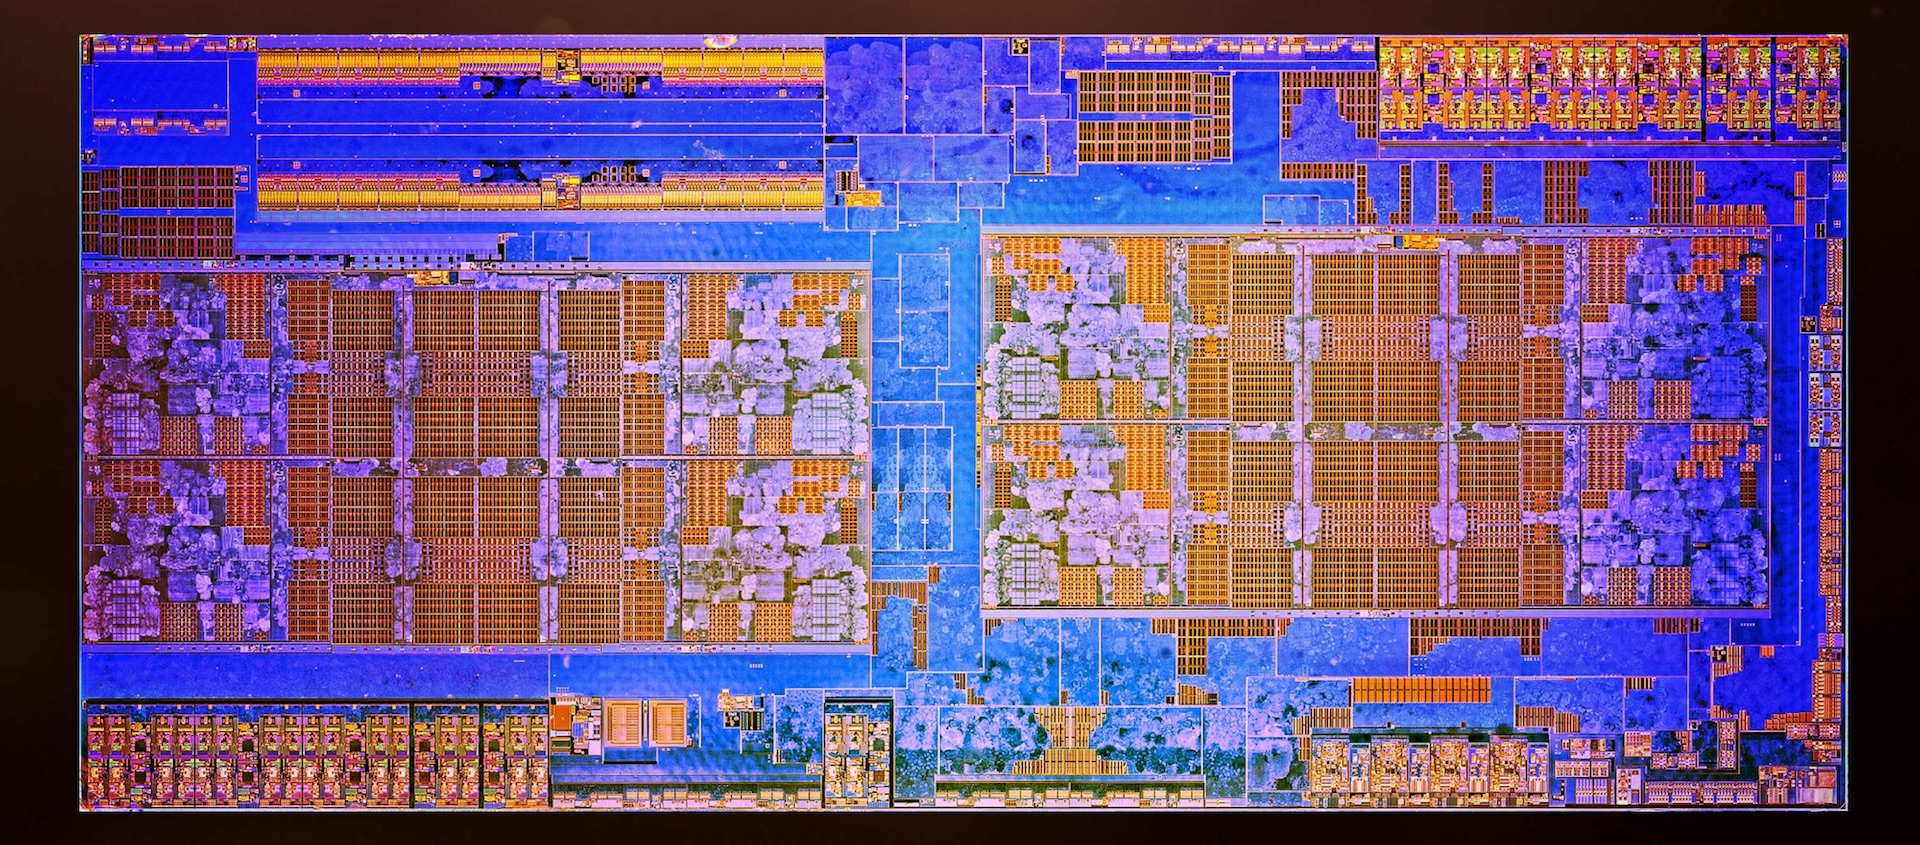
\includegraphics[width=0.7\textwidth]{ryzen-die.jpg}

\end{frame}

\begin{frame}
  \frametitle{Introduction}
  \framesubtitle{Ordres de grandeurs économiques en 2020}

\begin{itemize}
\item investissement pour la R\&D, la fabrication, l'usine pour un microprocesseur haut de gamme: dix milliards de US\$
\item nombre de transistors par puce: milliard (sur quelques centimètres carrés)
\item prix de vente (après test): environ mille dollars / pièce (milliers)
\item taux de rendement: quelques pourcents, la plupart des puces sont défaillantes
\item taux de panne par porte : moins d'une défaillance par heure
\item consommation énergetique du numérique: quelques pourcents de la production électrique française
\item prix de vente d'un ordinateur: centaines d'euros.
\item plusieurs "ordinateurs" par habitant (microcontrôleurs, informatique embarquée, téléphones portables, datacenters)
  \item productivité d'un développeur: quelques dizaines de milliers de ligne de code source par an.
\end{itemize}
\end{frame}

\begin{frame}
  \frametitle{Introduction}
  \framesubtitle{Ordres de grandeurs technologiques en 2020}
 
\begin{itemize}
\item 8 c{\oe}urs de processeur à 3GHz
\item mémoire cache: 16 Mo (accès 10ns, bande passante 0,5To/s)
\item taille mémoire RAM d'un ordinateur : 32 Goctets
\item temps d'accès RAM: 200 ns
\item bande passante RAM: centaine Mo/seconde
\item taille disque SSD : un téra-octets
\item puissance thermique dissipée en charge: 250W
\item temps d'accès SSD: 50 microsecondes pour un bloc de 4Ko.
\end{itemize}

\end{frame}

\begin{frame}

  \frametitle{Introduction}
  \framesubtitle{Vue interne d'un ordinateur de bureau en 2020}

\href{https://images.app.goo.gl/BMQxP7c4Zcyrh3XD7}{images.app.goo.gl/BMQxP7c4Zcyrh3XD7}

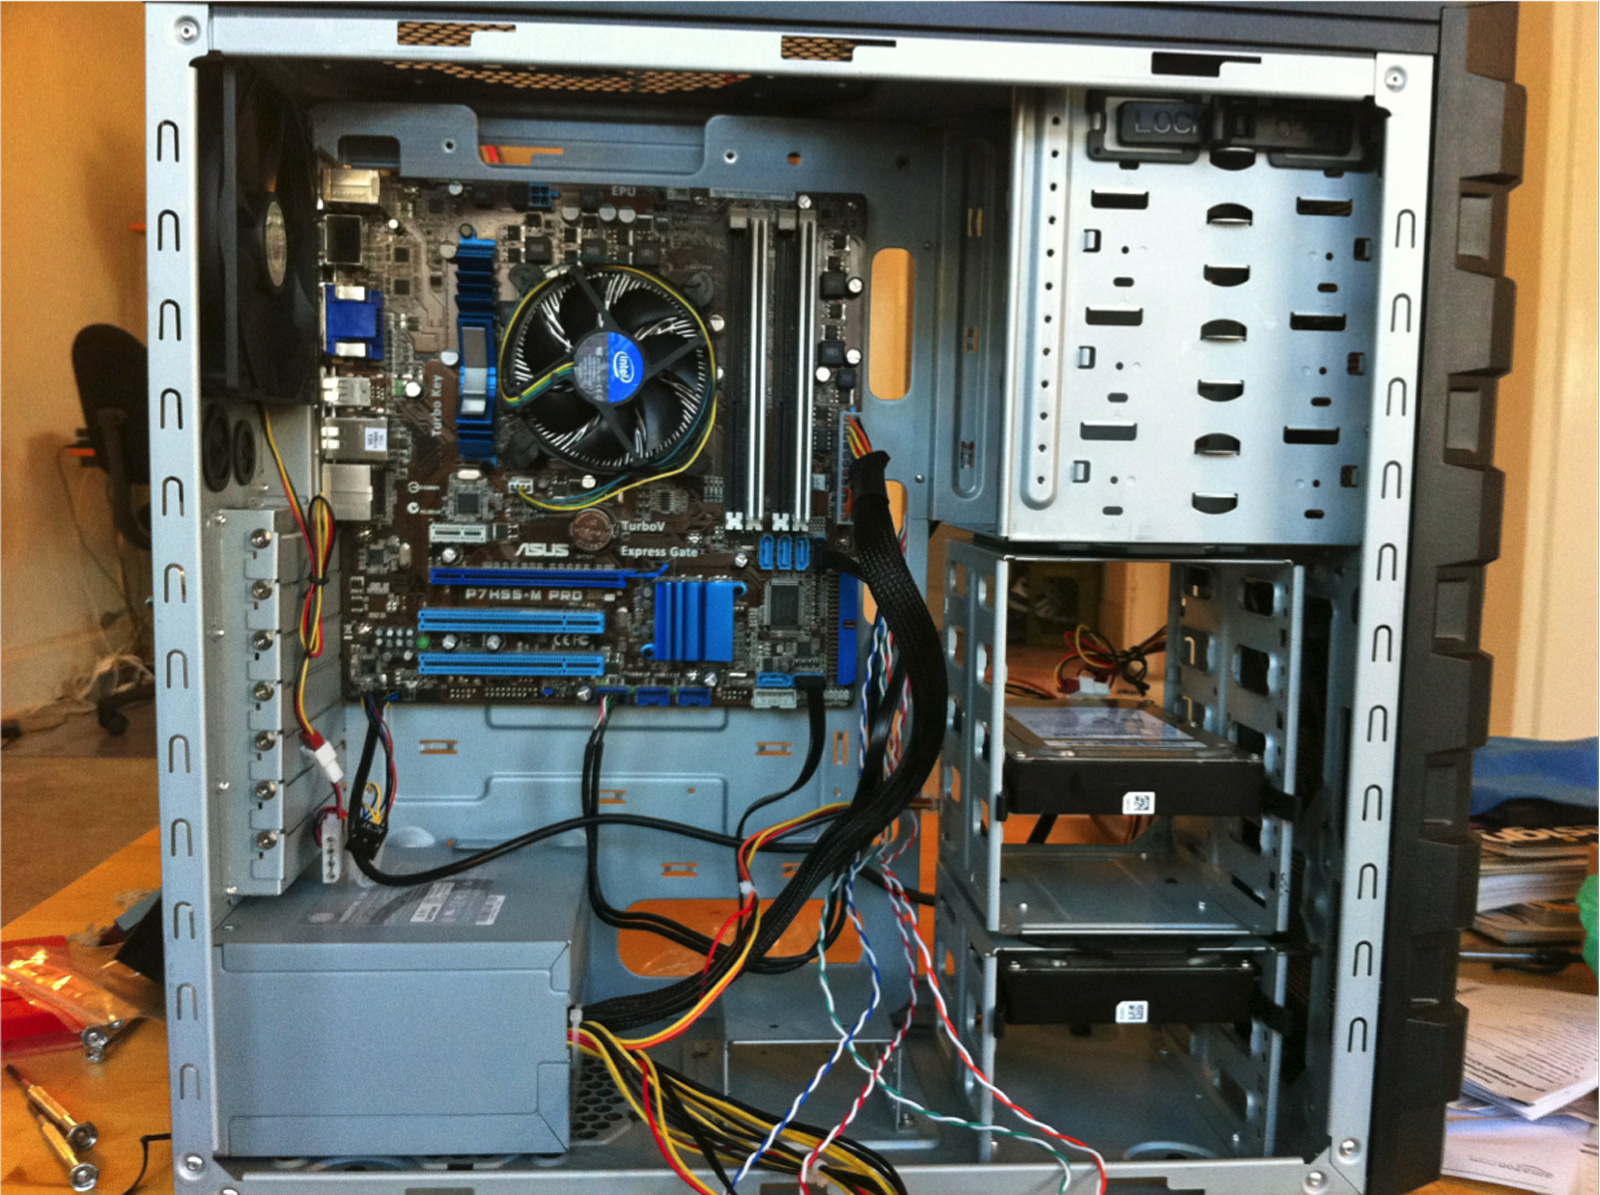
\includegraphics[width=0.66\textwidth]{interieur-ordinateur.png}
\end{frame}

%%%%%%%%%%%%%%%%%%%%%%%%%%%%%%%%%%%%%%%%%%%%%%%%%%%%%%%%%%%%%%%%%%%%%

\section{couches logicielles}

\begin{frame}
  \frametitle{Couches logicielles}
  \framesubtitle{Les différents types de logiciels}

\begin{itemize}

\item logiciel et langage de description des circuits (VHDL, SystemC)
\item firmware - interne à la souris (langage machine 8051), au disque dur, à la carte réseau
\item logiciel de démarrage (UEFI, BIOS): charge le système d'exploitation
\item noyau (par exemple Linux) du système d'exploitation, gère les fichiers
\item utilitaires systèmes (gestion du réseau, ...)
\item interface graphique ou navigateur Web
\item bibliothèques logicielles standard (\href{http://qt.io}{Qt}, \texttt{libc})
\item outils logiciels pour le développeur (compilateur)
\item logiciels applicatifs (bureautique) ou métiers (aéronautique)
\item scripts utilisateurs et fichiers de configuration
\item commandes, schémas de bases de données, langage d'imprimante

\end{itemize}
\end{frame}

\begin{frame}
  \frametitle{Couches logicielles}
  \framesubtitle{Aspects légaux (code pénal)}

  En France

  
  \begin{block}{article 323-1 et suivants du Code Pénal}

    \begin{relsize}{-0.5}
Le fait d'accéder ou de se maintenir, frauduleusement, dans tout ou
partie d'un système de traitement automatisé de données est puni de
deux ans d'emprisonnement et de 60 000 € d'amende.

Lorsqu'il en est résulté soit la suppression ou la modification de
données contenues dans le système, soit une altération du
fonctionnement de ce système, la peine est de trois ans
d'emprisonnement et de 100 000 € d'amende.

Lorsque les infractions prévues aux deux premiers alinéas ont été
commises à l'encontre d'un système de traitement automatisé de données
à caractère personnel mis en œuvre par l'Etat, la peine est portée à
cinq ans d'emprisonnement et à 150 000 € d'amende.
    \end{relsize}
  \end{block}
\end{frame}



\begin{frame}
  \frametitle{Couches logicielles}
  \framesubtitle{Aspects légaux (RGPD)}

  En Europe, obligation d'avoir le consentement éclairé et préalable
  pour tout traitement de données à caractère
  personnel. \textbf{\textcolor{red}{Règlement Général sur la
      Protection des Données}}

  Voir
  \href{https://donnees-rgpd.fr/definitions/rgpd-pour-les-nuls/}{\texttt{donnees-rgpd.fr/definitions/rgpd-pour-les-nuls}}, \href{https://www.laquadrature.net}{\texttt{www.laquadrature.net}} et \href{https://april.org/}{\texttt{april.org}} 
  pour en savoir plus.
\end{frame}

\begin{frame}
  \frametitle{Couches logicielles}
  \framesubtitle{Aspects légaux (copyright et logiciels libres, brevets logiciels, vente liée)}

  \textbf{copyrights logiciels et logiciels libres:} Voir
  \href{https://april.org/}{\texttt{april.org}} et
  \href{https://aful.org/}{\texttt{aful.org}} et
  \href{https://www.eff.org/}{\texttt{eff.org}} et
  \href{https://www.fsf.org/}{\texttt{fsf.org}} et
  \href{https://opensource.org/}{\texttt{opensource.org}} et
   \href{https://adullact.org/}{\texttt{adullact.org}} et
  \href{https://montpellibre.fr/}{\texttt{montpellibre.fr}} et
   \href{https://cecill.info/}{\texttt{cecill.info}} \textcolor{red}{\textit{etc...}}
  (ou votre juriste préféré)
    pour en savoir
    plus.

    \vspace{0.5cm}
    \textbf{Vente liée matériel + logiciel :} voir
    \href{https://non.aux.racketiciels.info/}{\texttt{non.aux.racketiciels.info}}
    et
    \href{https://bons-constructeurs-ordinateurs.info/}{\texttt{bons-constructeurs-ordinateurs.info}}
    
    \vspace{0.5cm}

    NB. \textbf{Ne pas inventer sa propre licence logicielle libre} sans
    assistance juridique: le droit est aussi complexe que
    l'informatique!
   
    \vspace{0.3cm}
 
    PS. Attention aux incompatibilités de licences logiciels entre composants logiciels
\end{frame}


\begin{frame}
  \frametitle{Couches logicielles}
  \framesubtitle{Aspects techniques et sociaux}

  \textbf{Code binaire} ou \textbf{code machine} \\
  Il est executé par l'ordinateur. Totalement illisible.

    \vspace{0.3cm}
  \textbf{Code source} \\
  Il est développé par l'informaticien et partagé avec d'autres. Contient plein de choses pour les humains, inutiles aux ordinateurs.

    \vspace{0.3cm}
  \textbf{Code intermédiaire} \\
  Des logiciels transforment le code source en code binaire, en passant par des representations intermédiaires. Dont le  \textbf{code objet}.
  
\end{frame}


\end{document}
%%%%%%%%%%%%%%%%%%%%%%%%%%%%%%%%%%%a%%%%%%%%%%%%%%%%%%%%%%%%%%%
%% Local Variables: ;;
%% compile-command: "./build.sh" ;;
%% End: ;;
%%%%%%%%%%%%%%%%%%%%%%%%%%%%%%%%%%%%%%%%%%%%%%%%%%%%%%%%%%%%%%%%
